\chapter{Method}
\section{Deep HAR}
\subsection{Approach}

%TODO
overview of pipeline (image)
motivation from authors of how and why they approached it this way
\cite{luvizon_2d/3d_2018}
based on their previous work in \cite{luvizon_human_2017}.

\subsection{Soft-argmax}
The authors propose an approach for computing the $x$ and $y$ coordinates from a joint heatmap using a method called \textit{Soft-argmax} \cite{luvizon_human_2017}.
After computing the Softmax $\Phi(h)$ of a joint heatmap $h$, $x$ and $y$ coordinates need to be regressed to be able to fine-tune the network in an end-to-end fashion since the regular argmax function is not differentiable \cite{luvizon_2d/3d_2018}.
This is achieved by computing the expectation in $x$ and $y$ regression on the probability map produced by the Softmax function.
In the implementation, the authros first define a fixed weight matrix for a convolutional layer in the following way:

\begin{figure}[htb!]
    \centering
    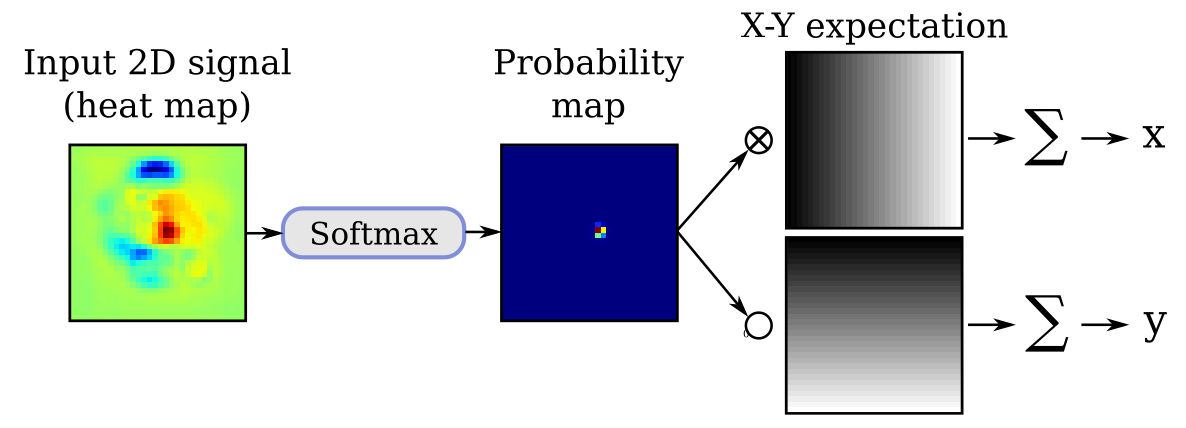
\includegraphics[width=0.6\textwidth]{softargmax_pipeline.png}
    \caption{The approach presented by the authors to regress $x$ and $y$ coordinates from heatmaps. First, they apply a Softmax. Then, they compute the expectation in both $x$ and $y$ direction using a \textit{2D ramp function}. Summation of the result then leads to the regressed coordinates. Image taken from \cite{luvizon_2d/3d_2018}. }
    \label{fig:softargmax_pipeline}
\end{figure}

\begin{equation}
    \bm{W}_{i,j,x} = \frac{i}{W}, ~ \bm{W}_{i,j,y} = \frac{j}{H},
\end{equation}

where $H, W$ refer to the width and height of the heatmap and $i,j$ are the coordinates for each element in the heatmap.
This leads to ramp functions for $x$ and $y$ dimension, which are visualized in \fref{fig:softargmax_pipeline}.
By convolving a part heatmap with both $\bm{W}_x$ and $\bm{W}_y$ the expectations are computed, leading to the regressed coordinate $(\psi_x(h), \psi_y(h)) = ((x_{exp}, y_{exp})$ (see \eref{eq:softargmax_conv}).

% TODO: output is [0,1], need to scale with width and height

\begin{equation}
    \label{eq:softargmax_conv}
    \psi_d(h) = \sum_{i=1}^W \sum_{j=1}^H \bm{W}_{i,j,d} \Phi(h_{i,j})
\end{equation}

The authors further prove that the Soft-argmax function is deferentiable by providing the derivative of $\psi_d(h)$:

\begin{equation}
    \frac{\partial \psi_d(h_{i,j})}{\partial h_{i,j}} = \bm{W}_{i,j,d} \frac{ exp(h_{i,j}) (\sum_{k=1}^W \sum_{l=1}^H exp(h_{k,l} - exp(h_{i,j}) ) } { ( \sum_{k=1}^W \sum_{l=1}^H exp(h_{k,l}) )^2 }
\end{equation}

Further, the authors argue that such a method for regressing $x$ and $y$ coordinates is more accurate and requires fewer training weights than directly regressing them using, for example, a fully-connected layer \cite{luvizon_human_2017}.
As proof, they compare their methods to other state-of-the-art methods which directly regress the coordinates, and observe that their approach consistently outperforms these approaches on the MPII benchmark.
Specifically, when comparing to the previously best approach for regressing pose by \cite{sun_compositional_2017}, the authors observe an overall increase in PCKh accuracy of $5.2$ percentage points from $86.4$ to $91.2$ percent.

For evaluating the accuracy of the Soft-argmax function, we performed two experiments.
For both experiments, an estimated coordinate $(x_{est},y_{est})$ was considered to be correct in comparison to the ground truth coordinate $(x_{gt}, y_{gt}$ if both $\lvert x_{est} - x_{gt} \rvert \leq 2$ and $\lvert y_{est} - y_{gt} \rvert \leq 2$, allowing for a $2$ pixel discrepancy between prediction and ground truth.
The reason for using a threshold of $2$ pixels was that the output of the Soft-argmax function are fractions of width and height with $(x_{frac}, y_{frac}) \in [0,1]$.
To compute the image coordinate, a multiplication with the width and height of the input image as well as a rounding step is necessary, possibly introducing rounding errors.

First, synthetic images of size $128 \times 128$ pixels were created.
For each $x,y$ position, a gaussian with mean $(x,y)$ and variance $v$ was placed.
Afterwards, the expectations were computed using the Soft-argmax function and compared to the ground truth mean value.
Performing this for each pixel coordinate and different variances $v$, it was observed that the Soft-argmax function accurately regressed the true expectation for small variances.
As the variance increases, the accuracy decreases, especially around the borders.
See \fref{fig:softargmax_variance_test} for a visualization, where violett pixels indicate a wrong prediction and yellow pixels indicate a correct prediction.
Second, synthetic joint heatmaps were generated by placing gaussians at the position of the ground truth label coordinates of a subset of the MPII dataset and the distance between the computed coordinates and ground truth coordinate was computed with different variance values $v$.
The experiment was conducted on $100$ random images from the MPII dataset.
See \tref{tab:softargmax_numeric_eval} for the mean accuracies achieved for variances $v \in \{1, 2, 5, 10, 20, 50 \}$.
%TODO: Talk about the results

\begin{table}[]
    \centering
    \scalebox{0.90}{%
    \begin{tabular}{|l|l|l|l|l|l|}
    \hline
    \textbf{$v=1$} & \textbf{$v=2$} & \textbf{$v=5$} & \textbf{$v=10$} & \textbf{$v=20$} & \textbf{$v=50$} \\ \hline
    0.01 & 0.01 & 0.01 & 0.01 & 0.01 & 0.01 \\ \hline 
    \end{tabular}}
    \caption{Mean average accuracy of Soft-argmax when detecting ground truth coordinates from synthetic joint heatmaps.} %TODO: Talk about results here too
    \label{tab:softargmax_numeric_eval}
\end{table}

%TODO: Small evaluation of the results of both experiments
This suggests that the Soft-argmax function requires that the heatmap used is highly accurate by itself and that the joints are not too near to the image border.

\begin{figure}[htb!]
    \centering
    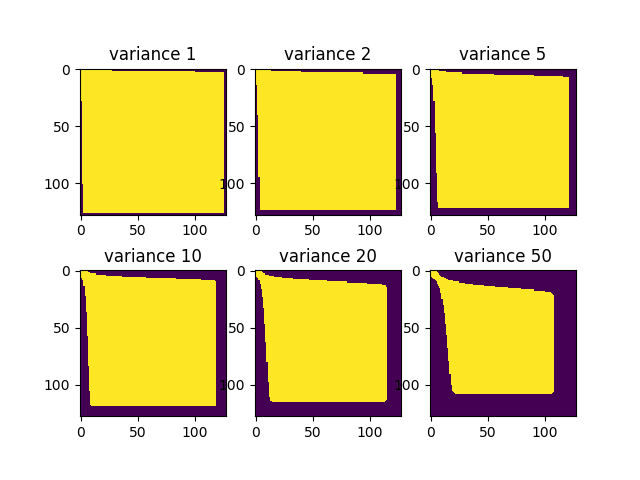
\includegraphics[width=0.7\textwidth]{softargmax_variance_test.png}
    \caption{Evaluation of the accuracy of the Soft-argmax function using synthetic data. Yellow pixels $i,j$ indicate where the Soft-argmax function correctly regressed the peak of the gaussian with mean value $i,j$, while violett indicates wrong predictions. Notice that the accuracy decreases when approaching the border of the image and when the variance is increasing. }
    \label{fig:softargmax_variance_test}
\end{figure}

\subsection{Architecture}
The architecture used by the authors can be divided into several blocks.
First, a feature extraction block, referred to as \textit{Stem}, is used to extract visual features from each frame of the input video.
Afterwards, these features are used to predict the joint heatmaps in the pose estimation block.
The heatmaps are then used to compute the $x$ and $y$ coordinates of the joint positions using the Soft-argmax function.
Then, the network splits into two action recognition pipelines.
In the first pipeline, further referred to as \textit{Pose-based action recognition}, the pose coordinates for all frames in the video clip are aggregated into a matrix and the action is predicted on this matrix.
In the second pipeline, further referred to as \textit{Appearance-based action recognition}, the image features from the \textit{Stem} block are aggregated in a similar fashion to the \textit{Pose-based action recognition} into a matrix, which is also used to predict the performed action.
Finally, both intermediate action predictions are combined to form the final prediction.
Throughout the entire network, the authors use the ReLU activation function.
See \fref{fig:luvizon_overview} for a visualization of the network and its separate components.

\begin{figure}[htb!]
    \centering
    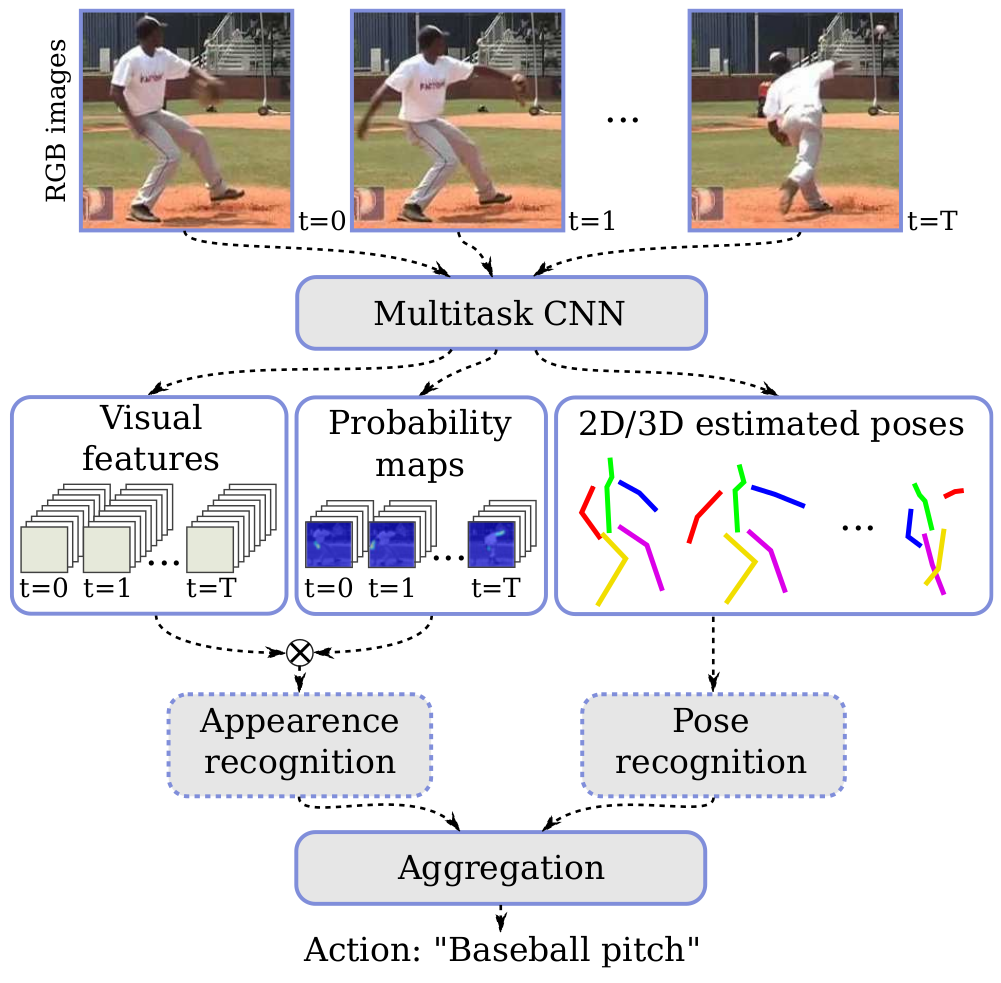
\includegraphics[width=0.6\textwidth]{endtoend-concept.png}
    \caption{High level visualization of the network used by \cite{luvizon_2d/3d_2018}. The images features and poses are computed frame-by-frame. The output is then passed to the appearance and pose recognition subnetworks, where they are jointly processed to predict the action of the video clip. Image taken from \cite{luvizon_2d/3d_2018}.}
    \label{fig:luvizon_overview}
\end{figure}

\subsubsection{Feature extraction (Stem)}
The authors base their feature extraction network off of the \textit{Inception v4} network proposed by \cite{szegedy_inception-v4_2017}.
One addition the authors made was to use a final \textit{depthwise separable convolutional layer} at the end of the network.

A \textit{depthwise separable convolution} \cite{sifre_rigid-motion_2014} \cite{chollet_xception:_2017} used to reduce the number of parameters and matrix multiplications needed for convolutional layers with many channels.
Consider an input matrix (like an RGB image) to a convolutional layer of size $n \times n \times p$, where $p$ indicates the number of channels.
Without loss of generality, a square input as well as a square kernel size is assumed.
If a regular convolutional layer is used, and the desired number of output channels is given by $m$ with $m \gg p$, then one approach is to use $m$ kernels in the convolutional layer of size $a \times a \times p$.
This results in $a^2 * p * m$ parameters of the convolutional layer which need to be learned.
In a depthwise separable convolutional layer, two convolutional layers are used after one another, referred to as the \textit{depthwise convolutional layer} and \textit{pointwise convolutional layer}.
The \textit{depthwise convolutional layer} uses $p$ filters of size $a \times a \times 1$ to process the input matrix one channel at a time.
Afterwards, the \textit{pointwise convolutional layer} uses $m$ filters of size $1 \times 1 \times p$.
This results in $$p * m + p * a^2 \Leftrightarrow p * (m + a^2)$$ learnable parameters for both convolutional layers, drastically reducing the number of parameters.
It is then easy to see that $$p * (m + a^2) \ll p * m * a^2.$$
Additionally, the number of matrix operations needed to compute the convolution is reduced significantly as well.
Let $b$ be the number of convolutions performed on either $x$ or $y$ dimension on an matrix of size $n \times n$ using a kernel of size $a \times a$.
The number of matrix convolutions necessary in a regular convolutional layer is equal to $a^2 * b^2 * p * m$.
In a depthwise separable convolutional layer, the number of multiplications reduces to $a^2 * b^2 * p $ for the depthwise and $b^2 * m * p$ for the pointwise convolutional layer.
This results in $$a^2 * b^2 * p + b^2 * m * p \Leftrightarrow b^2 * (a^2 * p + p * m) $$ convolutions.
To show that the number of convolutions needed is lower, it needs to be shown that $a^2 * p + p * m < a^2 * p * m$ (see \eref{eq:convolution_proof}).
The assumption in holds since $a \ll m$.

\begin{equation}
    \label{eq:convolution_proof}
    \begin{split}
        &a^2 * p + p * m < a^2 * p * m \\
        &\Leftrightarrow p * (a^2 + m) < p * a^2 * m \\
        &\Leftrightarrow a^2 + m < a^2 * m  
    \end{split}
\end{equation}

\begin{figure}[htb!]
    \centering
    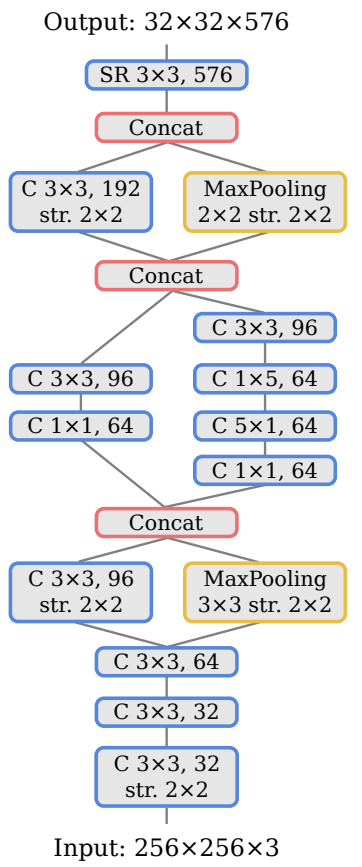
\includegraphics[width=0.3\textwidth]{luvizon_stem.png}
    \caption{The feature extraction network used in \cite{luvizon_2d/3d_2018}, also referred to as \textit{Stem}. Each RGB frame of the video is resized to $256 \times 256 \times 3$. \textit{SR} referres to a \textit{depthwise separable convolution}. The extracted features are of size $32 \times 32 \times 576$. Image taken from \cite{luvizon_2d/3d_2018} supplementary material.}
    \label{fig:luvizon_stem}
\end{figure}

\subsubsection{Pose estimation}
For the pose estimation network, the authors build upon the work by \cite{newell_stacked_2016} (see \sref{sec:stacked_hourglass}).


\subsubsection{Pose-based action recognition}
joint representation
forward reference to "differerent representations" subchapter

\subsubsection{Appearance-based action recognition}

\subsection{Limitations}
pose estimation only on single images. NO TEMPORAL COMPONENT, only when using for action recognition.

\section{Extensions}

\subsection{Combination of Loss Functions}

\subsection{Different Representations of Pose}